\scanpage{121}
définissent des germes de sous-espaces \inserted{$D_x^i$} de $X$ en l'image $a$ de $x$ dans $X$, qui contiennent le germe défini par $(D_d,x)\longrightarrow(X,a)$. Ceci dit, on veut que ce dernier germe soit l'\uline{intersection} des germes $D_x^i$, \inserted{et} \unsure{q.} bien sûr que cette intersection soit transversale.

Cette axiomatique inclut des cas tels que
\figure{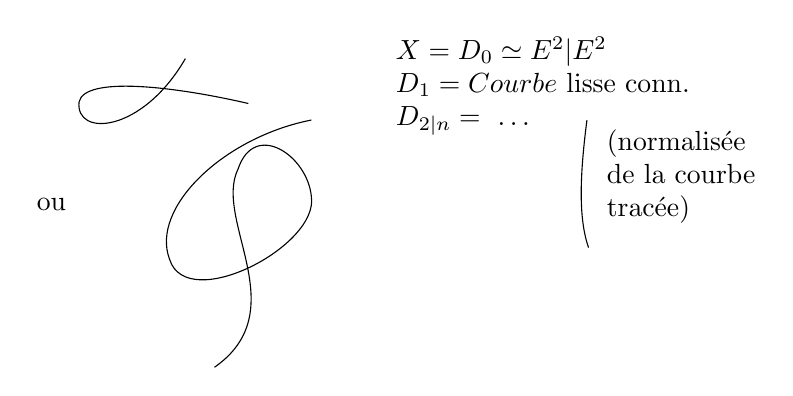
\begin{tikzpicture}[x=1cm,y=1cm]
\draw (1.0,3.5) .. controls (.45,2.55) and (-.40,2.50) .. (-.35,2.95) .. controls (-.28,3.28) and (.85,3.15) .. (1.80,2.93);
\node at (-.70,1.65) {ou};
\draw (2.60,2.72) .. controls (1.48,2.50) and (.55,1.60) .. (.80,.95) .. controls (1.02,.25) and (2.70,1.12) .. (2.60,1.75) .. controls (2.55,2.27) and (1.88,2.72) .. (1.67,2.10) .. controls (1.35,1.45) and (2.40,.30) .. (1.37,-.42);
\node[anchor=north west,align=left] at (3.55,3.90) {$X=D_0\simeq\unsure{\mathbb E^2|E^2}$\\$D_1=\unsure{\text{Courbe}}$ \uline{lisse} conn.\\$D_{\unsure{2|n}}=\varnothing\ \ldots$};
\draw (6.10,2.72) .. controls (6.00,1.95) and (6.00,1.45) .. (6.12,1.10);
\node[anchor=north west,align=left] at (6.23,2.72) {(normalisée\\de la courbe\\tracée)};
\end{tikzpicture}}
qui ne peut être décrit par la donnée d'un diviseur sur $X$, \deleted{lorsqu'on \unsure{en a choisi}}

\deleted{tel diviseur, dans}

L'opération de $\unsure{\mathfrak S_d|G_d}$ sur $\mathbb Z^d$ permet de construire sur $D_d$ un système local
\[
(183)\qquad T_d=D'_d\mathbin\wedge_{(\unsure{\mathfrak S_d|G_d})_{D_d}}(\mathbb Z^d)_{D_d},
\]
\deleted{\unsure{ou}} qui donne naissance à un groupe analytique (et $=$ algébrique) relatif sur $D_d$:
\[
(184)\qquad G_d=T_d\otimes_{\mathbb Z}\mathbb G_{m\,D_d}\simeq\unsure{D'_d|D_d^d}\mathbin\wedge_{(\unsure{\mathfrak S_d|G_d})_{D_d}}\mathbb G_m^d
\]
\deleted{Enfin} et $T_d$ s'interprète en termes de $G_d$ comme le syst. local des $\pi_1$ ou $H_1$ des fibres
\margin{120}
